% document type
\documentclass [12pt,oneside,a4]{report} % oneside
%\documentclass [12pt,twoside,openright,a4]{report} % twosided

% fixes
\usepackage{fixltx2e} % LaTeX patches, \textsubscript
\usepackage{cmap} % fix search and cut-and-paste in PDF

% language
\usepackage[english]{babel}
\usepackage[T1]{fontenc}
\usepackage[utf8]{inputenc}

% usability
\usepackage {makeidx}
\usepackage {float}
\usepackage {afterpage}

% formatting
\usepackage{amsmath}
\usepackage{url}
\usepackage{setspace}
\usepackage{hyperref}

\usepackage{verbatim}
\usepackage{fancyvrb}
\usepackage{mdwlist}
\usepackage{float,caption}

\usepackage{tikz}
\usetikzlibrary{fit, positioning}

\usepackage{algorithm}
\usepackage{algorithmicx}
\usepackage[noend]{algpseudocode}

\usepackage{graphicx}
\usepackage{ifpdf}
\usepackage{listings, textcomp, color, xcolor, caption}

\usepackage{todonotes}

\makeindex

\begin{document}
    %settings
    \onehalfspace
    %\normalsize{}
    \renewcommand{\baselinestretch}{1.1}

    \abovedisplayshortskip=0pt
    \belowdisplayshortskip=0pt
    \abovedisplayskip=4pt
    \belowdisplayskip=4pt

    \input source.tex

    \widowpenalty=500
    \clubpenalty=500

    %meta
    \title{ Parallel Pattern Discovery }
    \author{ Egon Elbre }

    \pagestyle{empty}

    \input title.tex

    \pagestyle{plain}
    \tableofcontents

    
\DefineVerbatimEnvironment{file}{Verbatim}%
    {fontsize=\small,
    fontfamily=tt,
    gobble=0,
    frame=single,
    framesep=2mm,
    baselinestretch=0.8,
    labelposition=topline,
    samepage=true}

\DefineVerbatimEnvironment{cmd}{Verbatim}%
    {fontsize=\small,
    fontfamily=tt,
    gobble=0,
    frame=none,
    framesep=5mm,
    baselinestretch=0.8}

% algorithm environment
\newcommand{\sym}{\mathcal}
\newcommand*\Let[2]{\State #1 $\gets$ #2}
\newcommand{\func}[2]{\textbf{fn}(#1)\{#2\}}

\algblockdefx[SPAWN]{Spawn}{EndSpawn}{\textbf{start workers}}{}

\algrenewcommand\algorithmicrequire{\textbf{Input:}}
\algrenewcommand\algorithmicensure{\textbf{Output:}}

% for representing tokens
\newcommand{\R}[1]{\colorbox{black!15}{\texttt{#1}}}
\newcommand{\cmdline}[1]{\colorbox{black!15}{\texttt{#1}}}

% defintions

%\theoremstyle{plain}% default
%\newtheorem{thm}{Theorem}[section]
%\newtheorem{lem}[thm]{Lemma}
%\newtheorem{prop}[thm]{Proposition}

\theoremstyle{definition}
%\newtheorem{defn}{Definition}[section]
%\newtheorem{conj}{Conjecture}[section]
\newtheorem{exmp}{Example}[section]

%\theoremstyle{remark}
%\newtheorem*{rem}{Remark}
%\newtheorem*{note}{Note}
%\newtheorem{case}{Case}

% todo things
\newcommand{\insertref}[1]{\todo[color=green!40,fancyline]{cite #1}}
\newcommand{\tow}[1]{\todo[inline]{write #1}}
\newcommand{\hmm}[1]{\todo[fancyline]{#1}}

\newcommand{\eg}{\todo[fancyline]{add examples}}
\newcommand{\WIP}{\todo[color=blue!40,inline]{Work in progress}}



\lstset{ %
    basicstyle=\scriptsize,
    breaklines=false,
    numbers=left,
    numberstyle=\tiny\color{black!80},
    stringstyle=\it,
    escapechar=@,
    columns=fixed
}

    \chapter{Introduction}

\section{Motivation and background}

Collecting new data has been increasing more rapidly than algorithms and
computer processing power. The average size of each dataset has also
been increasing. This suggests that the only way to keep up with
analysis is to parallelize algorithms.

One of main drivers of such large datasets is analysis
of genomic and proteomic sequences. Regularities in such data can 
give new insights into how these patterns form and how 
they are related to the other features of the data.

\todo[inline]{More on importance}

In this thesis we explore an algorithm for finding patterns and show how
abstractions can make it scalable and flexible, and simpler both in 
theory and implementation compared with non-abstract version.

\section{Pattern Discovery}

Pattern discovery is a research area aiming to discover unknown patterns
in a given set of data structures that are frequent and interesting according 
to some measure.

Since the discovery algorithms are highly dependent on the
data structures, that are being searched, the algorithm must be minimal
in the requirements on the dataset to be applicable as wide range as possible.
This also means that the patterns found must be dependent on the initial data.

\section{Structure of the thesis}

Basic idea is to select a basis algorithm. Abstrify away concretness of 
implementation to support flexibility. Use the flexibility to substitute 
concretness with parallel implementations.

\todo[inline]{Fix when structed}

First we introduce definitions of our data and patterns in Chapter 2. In
Chapter 3 we describe the general SPEXS algorithm as specified in Vilo et al.
In Chapter 4 we generalize and abstrify the algorithm to get a more flexible
and parallel algorithm. We will describe the implementation consideration of
flexible algorithms in Chapter 5 using the abstract SPEXS algorithm as an
example. Chapter 6 uses the implementation to show how it can be applied.
    \chapter{Definitions}
\label{c:definitions}

Pattern discovery is a research area aiming to discover unknown patterns in a given set of data structures that are frequent and interesting according to some measure. In this chapter we formally define necessary terms used in this thesis.

\section{Sequence and Dataset}

We use $\Sigma$ to denote the set of tokens in the dataset, an \emph{alphabet}. 
The \emph{size} of the alphabet is $|\Sigma|$. \emph{Tokens} can be numbers, 
letters, words or sentences - any symbol.

Any sequence $S=a_1 a_2 ... a_n, \forall a_i \in \Sigma$ is called a \emph{sequence} 
over the token set $\Sigma$. If the length of the
string is $0$, it is called an empty sequence or $\epsilon$.

\begin{exmp}
\R{ACGTGCCATC} is a sequence where $\Sigma = \{\R{A}, \R{C}, \R{G}, \R{T}\}$.
\end{exmp}

A \emph{dataset} is a collection of sequences.

\begin{exmp}
In a document sentences can be considered as a \emph{dataset}, where a single sentence is a \emph{sequences} and each word is a \emph{token} in the alphabet. Text \R{This is some example. This is an other example.} has sequences \{ [\R{This is an example}], [\R{This is an other example}] \} and the alphabet is $\Sigma =$ \{\R{this}, \R{is}, \R{an}, \R{example}, \R{other}\}.	
\end{exmp}

\section{Pattern}

Our aim is to discover repetetive and common structures in data. We call such structures \emph{patterns}. A generic way to define a \emph{pattern} is as a set of all the sub-structures it represents. This means we can say whether some data sub-structure is represented by a pattern.

The \emph{pattern structure} is usually dependent on the data-structures which it represents. For example sequence patterns are usually represented sequences, graph patterns are represented as graphs; but sequence patterns could also be represented as a graph.

We denote the set of structures that a pattern structure $p$ defines as $all(p)$. If $\alpha \in all(p)$, where $\alpha$ is a structure then we say that
structure $\alpha$ \emph{matches exactly} pattern $p$. We say that $\alpha$ \emph{matches} $p$ if any of structure $all(p)$ is a sub-structure of $\alpha$.

In this thesis we only consider sequential pattern structures and use \emph{pattern} to mean \emph{sequential pattern structure}. We represent such patterns with regular expressions\insertref{regexp}. 

\tow{about regexps}

\emph{Pattern size} is the length of the pattern sequence.

\begin{exmp}
\R{.[AT]} is a pattern of size 2 and denotes a set 
\{ \R{AA}, \R{AT}, \R{CA}, \R{CT}, \R{GA}, \R{GT}, \R{TA}, \R{TT}\}; it matches \R{CCTC} and exactly matches \R{AT}.	
\end{exmp}

We denote the set of all pattern $p$ \emph{matches} in a dataset $D$ as $matches(p, D) = \{ match(p, \alpha) | \alpha \in D, matches(p, \alpha) \}$.

\section{Query}

We need to somehow understand where given pattern $p$ is located in a dataset $D$. This compound structure $q = <D, p, matches(p, D)>$ is called a \emph{query}.

\begin{exmp}
Let out dataset be $D = [ \text{\R{ACGT}}, \text{\R{TXCGA}} ]$ and our pattern be $p = \text{\R{C.}}$. The corresponding query is $<D, p, \{ [1,3], [2,4]\}>$, which means that the pattern $p$ ends in sequence 1 at position 3 and in sequence 2 at position 4.
\end{exmp}

\subsection{Query features}

When we talk about how "interesting" a pattern is, we are actually evaluating the query, since the pattern requires a context where it can be "interesting".

Queries can have different properties: length, number of matches in the dataset, pattern textual representation etc. Such properties can be represented by a function that take a query as an input and return the property. Formally a \emph{query feature} is a function $f: Query \mapsto Any$.

We also need to see how "interesting" one query is compared to the others. \emph{Query interestingness} is a function $f: Query \mapsto Value$ where the $Value$-s are well-ordered. This gives a measure to compare two different queries. Often we can represent such interestingness measures as a real number.

We should also be able to somehow specify criterias for query. \emph{Query filter} is a function $f: Query \mapsto Boolean$ and shows whether the query matches the criteria.

\begin{exmp}
Pattern occurences in a document is a interestingness measure. Whether query pattern is at least 3 tokens is a query filter.
\end{exmp}

\section{Pool}

\emph{Pool} is an abstract datatype for a collection of queries. The pool allows queries to be stored. The only operations that pool must provide is "push", for adding a query, and "pop", for getting a query.

\begin{exmp}
Stacks and queues both satisfy the pool requirement. We could also define a pool that stores the queries on the disk; also it could pack or reorder the queries for performance reasons.
\end{exmp}

\section{Pattern Discovery}

In this thesis \emph{pattern discovery} is a process of finding the most interesting subset, according to a query interestingness, of sequential patterns, that conform to some criteria, in a sequence dataset.

\begin{exmp}
Let our search problem be "Finding most common nucleotide patterns that are at least 3 nucleotides long from a shotgun sequencing output.", then \emph{most common} defines our interestingness measure. \emph{At least 3 nucleotides} is the pattern subset criteria. \emph{Sequencing output} is our dataset and \emph{nucleotides} define the token alphabet.
\end{exmp}
    \chapter{Overview\hmm{better title needed}}
\label{c:algorithms}

\WIP

In this chapter we give a overview of different algorithms used for pattern discovery.

\hmm{Reorganize somehow}

\section{Algorithms}

Overview of different combinatorial algorithms.

\subsection{SPEXS}

SPEXS is an pattern discovery algorithm described in "Pattern Discovery from Biosequences"\cite{spexs}. This algorithm finds patterns from a sequence. We take this as our basis for developing a new parallel algorithm. In this chapter we describe original algorithm so that we can later show the changes made to this algorithm.

We describe the general representation of the SPEXS algorithm. 
The original algorithm was as follows:

\todo[inline]{move algorithm to generalization}

\begin{algorithm}[H]
	\caption{The SPEXS algorithm}
\begin{algorithmic}[1]
	\Require{String $S$, pattern class $\sym{P}$, output criteria, search order, and fitness measure $\sym{F}$}
	\Ensure{Patterns $\pi \in \sym{P}$ fulfilling all criteria, and output in the order of fitness $\sym{F}$}

	\State Convert input sequences into a single sequence
	\State Initiate data structures

	\Let{Root}{new node}
	\Let{Root.label}{$\epsilon$}
	\Let{Root.pos}{(1,2,...,n)}
	\State enqueue($\sym{Q}$, Root, order)

	\While{$N \gets$ dequeue($\sym{Q}$)}
		\State Create all possible extensions $p \in \sym{P}$ of $N$ using $N$.pos and $S$
		\For{ extension $p$ of $N$}
			\If{pattern $p$ and position list $p$.pos fulfill the criteria}
				\Let{$N$.child}{$p$}
				\State calculate $\sym{F}(p,S)$
				\State enqueue($\sym{Q}$,$p$,order)
				\If{$p$ fulfills the output criteria}
					\State store $p$ in output queue $\sym{O}$
				\EndIf
			\EndIf
		\EndFor
	\EndWhile
	\State{Report the list of top-ranking patterns from output queue $\sym{O}$}
\end{algorithmic}
\end{algorithm}

The main idea of the algorithm is that first we generate a 
pattern and a query that matches all possible positions in 
the sequence. We then put this query into a queue for extending.
Extending a query means finding all queries whose patterns length
is longer by 1. If any of the queries is fit, by some criteria,
it will be put into the main queue, for further extension, 
and output queue for possible output.

\subsection{TEIRESIAS}

TEIRESIAS\cite{TEIRESIAS} is an algorithm for the discovery of rigid patterns in biological sequences. \tow{more}

TEIRESIAS operates in two phases: scanning and convolution. Scanning phase identifies elementary patterns that are frequent. During convolution these elementary patterns are combined to make larger patterns.

This method is a divide and conquer method to only consider frequent patterns.

patterns with any symbol 

\tow{more} 

\subsection{Verbumculus}

Verbumculus\cite{Verbumculus} is...

statistical analysis, pattern matching

no complex patterns

\tow{more}

\subsection{MobyDick}

MobyDick\cite{MobyDick}...
statistical prediction of frequent

no complex patterns

\tow{more} 

\subsection{RSAT}

RSAT\cite{RSAT} is ...

matrix based pattern

\tow{more}

\subsection{Other}

\cite{NetworkMotifsDiscovery, GenericMotifSequential}

\section{Reviews}

\cite{CombinatorialSubtle, SurveyDNAMotif, SurveyMotifDiscovery}

\tow{about some reviews}

\section{Problems}

\WIP

Algorithms are fixed and hard to extend with new pattern types, structures and optimizations. Generalization usually comes at the cost of performance and complexity. \tow{more}

Sequential algorithms do not take advantage of multicore processors. \tow{more}

Data that exceeds computer memory can't work efficiently... can't be distributed efficiently. \tow{more}
    \chapter{Abstractification}

In this chapter we discuss the general structure of the new algorithm.

\section{Algorithm}

The algorithm in a more convetional view is:

\begin{verbatim}
func SPEXS(dataset, in, out, extender, extendable, outputtable, postprocess) {
	q := NewEmptyQuery(dataset)
	in.Put(q)
	while( !in.Empty() ) {
		q := in.Take()
		extended := extender(q)
		foreach qx in extended {
			if extendable(qx)
				in.Put(qx)
			if outputtable(qx)
				out.Put(qx)
		}
	}
}
\end{verbatim}

When the algorithm starts we create an empty pattern query and put 
into the in pool. The in pool contains querys whose patterns
should be further examined.

We pick a query from the in pool for extending. The extending means
generating all querys whose pattern is larger by one. There can be
several such querys.

If any of the querys should be further examined as defined by the
extendable filter, it will be put into the in pool.

If the query is fit for output we as defined by the outputtable filter,
it will be put into the out pool.

If we extend each pattern at each step by one we guarantee that we
examine the all patterns that conform to our criteria.

\section{Pools}

Pool is an abstract datatype for a collection of querys. The pool
allows querys to be put into it and taken from it, also we can
ask whether the pool is empty or not.

It has no guarantees on how the querys are stored internally and
in which order they are taken out.

In practice this means we can use any collection such as list, set,
queue as a pool. This gives us different performance characteristics.

\section{Filtering}

Filtering allows us to dramatically reduce the number of querys
we have to look at. It also allows to select only interesting patterns by
some criteria.

If we have interestingness measure we can create filter from it by
defining it's minimum or maximum value. One very usefule example 
would be a filter for limiting the pattern length.

By separating the extension and output filter, as opposed to SPEXS, 
we can still limit output without affecting the extension process.
For example if we wish to see only patterns of length 3 we cannot do
it with one filter. Since we need to extend patterns of length 0, 1 and 2.

\section{Extending}

The extending process is at the core of the algorithm. 
We shall look at how we can deal with different types.

The extending method is:

\begin{verbatim}

func extender(query) {
	// find all next positions
	nexts = new collection
	foreach pos in query.Matches {
		token, set of nexts = next(pos)
		nexts.add({token, set of nexts})
	}

	// group positions by the token
	matches = new map token => pos
	foreach x in nexts {
		matches[x.token].add(x.pos)
	}

	// make new querys from the matches
	result := new query collection
	foreach token, positions in matches {
		q := NewQuery( query.Pattern + token, positions )
		result.add(q)
	}

	return result
}

\end{verbatim}

\subsection{Sequences}

The simplest of the extensions are just sequences.

Let's consider a sequence ACGCCGATCGC and a pattern CG.

Diagram of the ACG.CCG.ATCG.C and query for that pattern.

Next positions step is finding ACG.[C]CG.[A]TCG.[C].

Grouping is [C] ==> CGC, [A] => CGA.

\subsection{DFAs}

Since we want to find more interesting patterns we can add more
information to the sequence DFA. Such as a star expression.

Same sequence with star paths.

\subsection{Groups}

Although we can add the group information to the DFA, it is more
performant to use the information gathered from the extension
of non-groups.

A[CG].Positions = AC.Positions union AG.Positions

\subsection{Other}

There maybe several other extensions to the regular expressions.

Questionable position:

AC?.Positions = A.Positions + AC.Positions
    \chapter{Parallelization}

Here we describe how we can partition the algorithm to support parallelism.
A proof of concept for fully parallelized code can be seen in appendix A.

\section{Process}

The main process of the algorithm as described by dataflow diagram.\cite{Kahn74,Lee95}

\begin{figure}[H]
	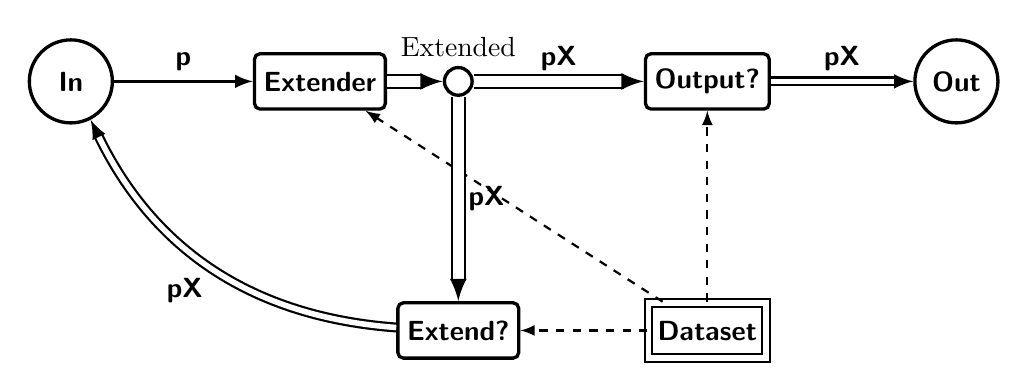
\begin{tikzpicture}[auto]
	\tikzstyle{pool} = [
		draw, very thick, fill=white, 
		circle,
		minimum height=3em, minimum width=3em, 
		node distance=9em, font={\sffamily\bfseries}];
	\tikzstyle{temppool} = [
		draw, very thick, fill=white, 
		circle,
		minimum height=1em, minimum width=1em, 
		node distance=5em, font={\sffamily\bfseries}];

	\tikzstyle{filter} = [
		draw, very thick, fill=white, 
		rectangle, rounded corners=0.2em,
		minimum height=2em, minimum width=4em,
		node distance=9em, font={\sffamily\bfseries}];
	\tikzstyle{extender} = [
		draw, very thick, fill=white, 
		rectangle, rounded corners=0.2em,
		minimum height=2em, minimum width=4em,
		node distance=9em, font={\sffamily\bfseries}];

	\tikzstyle{dataset} = [
		draw, thick, fill=white, 
		rectangle, double, double distance=2pt,
		minimum height=2em, minimum width=4em,
		node distance=9em, font={\sffamily\bfseries}];

	\tikzstyle{take} = [
		very thick, ->, >=latex,
		text centered, font={\sffamily\bfseries}];
	\tikzstyle{chan} = [
		thick, ->, >=latex, double, double distance=4pt,
		text centered, font={\sffamily\bfseries}];
	\tikzstyle{filtered} = [
		thick, ->, >=latex, double, double distance=2pt,
		text centered, font={\sffamily\bfseries}];
	\tikzstyle{needs} = [
		thick, ->, >=latex, dashed,
		text centered, font={\sffamily\bfseries}];

	\node[pool] (in) {In};
	\node[extender, right of=in] (ext) {Extender};
	\node[temppool, right of=ext, label=above:Extended] (exts) {};
	\node[filter, right of=exts] (outable) {Output?};
	\node[filter, below of=exts] (extable) {Extend?};
	\node[pool, right of=outable] (out) {Out};

	\node[dataset, right of=extable] (dataset) {Dataset};
	\draw[needs] (dataset) to (ext);
	\draw[needs] (dataset) to (outable);
	\draw[needs] (dataset) to (extable);

	\draw[take] 
		(in) to node{p} (ext);
	\draw[chan]
		(ext) to (exts);
	\draw[chan] 
		(exts) to node{pX} (outable);
	\draw[chan] 
		(exts) to node{pX} (extable);
	\draw[filtered, bend left] 
		(extable) to node{pX} (in);
	\draw[filtered]
		(outable) to node{pX} (out);
\end{tikzpicture}

\end{figure}

\todo{use proper syntax for dataflow diagrams}

Here we can see that the only dependence between query extending is the original dataset.

\section{Adding Nodes}

We can have multiple \emph{in} nodes if the \emph{extender} knows from where to fetch the \emph{querys}, which would require an additional scheduler.

This means that we can run several \emph{extenders} in parallel without effecting the overall process. Although we introduce a source for indeterminism.

\section{Extending}

Since much of the work is done in \emph{extender} we should also try to parallelize it as well:

\begin{algorithm}[H]
	\caption{Parallel Extender with Group optimization}
\begin{algorithmic}[1]
	\Require{Query $q$, function $next : \sym{I} \rightarrow [(\sym{I}, \sym{P})]$ }
	\Ensure{Set of querys that have been extended by one step}

	\Statef{ nexts \gets map(next, positions(q.matches)) }
	\Statef{ matches \gets groupBy(fst, nexts) }
	\Statef{ result \gets map(queryMaker(q), matches) }
	\Statef{ optimized \gets map( (x) \rightarrow (union(matches(x))), groups) }
	\Statef{ return union(result, optimized)}
\end{algorithmic}
\end{algorithm}

\todo[inline]{figure out how to make it readable}

\section{Dataset partitioning}

Since the dataset itself can be large it would be useful to divide it into parts. 

As we can see the extender only needs that sequences are intact, hence we can do the extension on partitioned dataset.

If we look at where we need synchronization points if we partition 
the dataset. Whole parts of extension still apply for parts of dataset.

The whole dataset is required only for filtering, since even one of the simplest operations ("counting matches in dataset") requires full knowledge of all matches over the dataset. But many such features can be calculated on sharded dataset with map-reduce.

\todo[inline]{example how to do counting}

There are also operations that require presence of all information or extended synchronization. One of the examples implemented in SPEXS is finding minimal p-value by splitting the data.

\todo[inline]{explain the optimal finding}

\section{Parallelized Process}

Applying these techniques we get a parallel dataflow:

\missingfigure{fully parallelized dataflow diagram}
    \chapter{Implementation}

The actual implementation may need to diverge from the abstract
defintion of the algorithm for practicality, simplicity or
performance reasons.

Many of the operations can be optimized for some particular
subset of datasets and features.

In this part we will use actual code from the program to show 
the implementation. For an introduction to the language 
Go that has been used see the appendix.

\section{Algorithm}

The algorithm was implemented as:

\begin{verbatim}
type Setup struct {
	Db  *Database
	Out Pooler
	In  Pooler

	Extender Extender

	Extendable  Filter
	Outputtable Filter

	PostProcess PostProcess
}

func Run(s *Setup) {
	prepareSpexs(s)
	for {
		p, valid := s.In.Take()
		if !valid {
			return
		}

		extensions := s.Extender(p)
		for _, extended := range extensions {
			if s.Extendable(extended) {
				s.In.Put(extended)
			}
			if s.Outputtable(extended) {
				s.Out.Put(extended)
			}
		}

		if s.PostProcess(p) != nil {
			break
		}
	}
}
\end{verbatim}

Setup is a structure designed to hold the full setup of the algorithm.
The algorithm is very similar to the algorithm described in the theoretical
part, with the slight addition of PostProcess.

\section{Architecture}

The main criteria for designing program have been described in D. Parnas
paper On the Decomposition of Programs. It suggests decomposing into
isolated units and parts that are likely to change together.

We chose the following decomposition:

\begin{verbatim}
	Configuration
	Dataset reader
	Setup
	Algorithm
		Sets
		Pools
		Extenders
		Features
		Filters
	Printer
\end{verbatim}

\subsection{Configuration}

One problem with flexible algorithms is that they a lot of ways to be run.
This often would need having tens or hundereds of program flags.
To avoid this problem we decided to use a json file for the program
configuration.

Example Configuration.

The problem with only using a json file is that when running from
command line it may be more comfortable using flags. To solve this problem
we added replacement strings into the json files that can be given in as
a program argument.

\begin{verbatim}
	"Datasets" : {
		"fore" : { "File" : "$input$"
	...
\end{verbatim}

When using spexs2 --conf conf.json input=filename the input will be
replaced by filename. Also there is optional default value if
one wasn't given.

\subsection{Dataset reader}

One of the most likely things to change is the input format. As an 
example we can have different delimiters. By adding this separation
immediately we can avoid the future problem of trying to support multiple
formats.

\subsection{Datasets}

We also may need to process several files. This means that we should
treat each file as a separate entity and allow calculate features
only on part of the dataset.

\subsection{Setup}

There are a lot of ways to setup the program. This allows us to separate
the initialization all of the structures necessary for the algorithm
from the algorithm itself.

\subsection{Algorithm}

This is an obvious separation. This is the main driver of the algorithm
and shouldn't know anything about the rest of the setup. Also there
are two versions of the algorithms one parallel the other not.

\subsection{Sets}

Since we need a collection how to store the matching positions it suggests
the need for a set datatype.

\subsection{Pools}

There can be different performance characteristics when using a particular
implementation. Most importantly to support parallelism they should
be ideally lock-free, but we can use locked version as well.

For the pools we have several choices: lifo, fifo or priority.

If we use a fifo queue as the in pool the algorithm does a breadth first
search of patterns. This can be problematic since we would need a lot of
memory to hold all the patterns in memory.

A lifo queue for in pool is a more reasonable choice for memory problems since we need
to hold less patterns in memory.

A priority queue suits for the out pool since we can easily then
use some feature to sort the queue and choose only a limited amount.

\subsection{Extenders}

As we saw in the theoretical part there are a lot of ways to extend
the query. Hence it is reasonable to decompose into a separate piece from
the algorithm.

\subsection{Features}

We can use these features to find out something about the query.
They each feature is defined as:

\begin{verbatim}
type Feature func(q *Query) (float64, string)
\end{verbatim}

Most of features are in $R$, but for some there
is some extended information that we may wish to know - hence
the need for additional string value. One of the simplest
is Pattern representation.

Also many of the features are defined in terms of multiple datasets.
We can use a closure to easily define a more generic feature.

Example:

\begin{verbatim}
func Matches(dataset []int) Feature {
	return func(q *Query) (float64, string) {
		matches := countf(q.Pos, dataset)
		return matches, ""
	}
}
\end{verbatim}

Here the Matches function creates a feature function defined
for dataset.

We can use the name in the configuration file as "Matches(fore)".

\subsection{Filters}

If a feature returns a floating point value we can easily turn that
into a filter by specifying a minimum or/and maximum value.

For example to give a lower and higher limits to some feature:

\begin{verbatim}
func featureFilter(feature Feature, min float64, max float64) Filter {
	return func(q *Query) bool {
		v, _ := feature(q)
		return (min <= v) && (v <= max)
	}
}
\end{verbatim}

Of course there are some filters that cannot be defined by features hence
there is still possibility to make separate filters. Such as disallowing
star symbol in the beginning of the pattern.

\subsection{Printer}

Although we use a general formatting there may be a need to save into
several files or output some extended information of the query.

\section{Debugging}

Debugging is a important part of development process hence the need for
more information how the algorithm is working.

Often this is resolved by adding some debug statments:

\begin{verbatim}
	for i := 0; i < 100; i += 1{
		printf("picking")
		a := pick()
		printf("picked %v", a)

		printf("picking")
		b := pick()
		printf("picked %v", b)
		
		out.put(a + b)
	}
\end{verbatim}

This can be harmful to the readability of the code. To fix this debugging 
problem we use closures.

\begin{verbatim}
	type PickFunc func() Thing
	func debuggable(fn PickFunc) PickFunc {
		return func() Thing {
			printf("start")
			p := fn()
			printf("picked %v" p)
			return p
		}
	}

	pick = debuggable(pick)
	for i := 0; i < 100; i += 1{
		a := pick()
		b := pick()
		out.put(a + b)
	}
\end{verbatim}

As we can see the algorithm implementation is much more readable.


    \chapter{Applications and experimental results}

Here we show example uses for the program:

\section{DNA sequences}

Make an example.

\section{Protein sequences}

Make an example.

\section{Text mining}

Make an example.


    \chapter{Conclusions}
\label{c:conclusions}

In this thesis we analyzed how to develop a parallel pattern discovery algorithm. We showed how we can take an already existing algorithm and parallelize it by generalizing, decomposing and then reifying. Finding the general idea of the algorithm can simplify the algorithm and provide more intuitive way of interpreting it. Decomposing allows us to talk about separate parts of algorithm and modify them without affecting the general idea of the algorithm. If we have an abstract algorithm we can substitute those parts with parallel structures and algorithms.

As a practical part we implemented a parallelized algorithm based on \emph{spexs}\cite{spexs}. We discussed several problems of implementing an algorithm and interesting approaches to these problems. The program has been designed to be easily extendable for different inputs, filters and interestingness criteria. We discussed different possible uses for the implementation and analyzed the performance gained from parallelization.

Further work on \emph{spexs2} should investigate the best configurations for different applications. We discussed that \emph{spexs2} could be made to find tree and graph patterns, it could be an interesting research topic.

Approaches suggested in this thesis could be used to generalize and parallelize other algorithms. Finding generic algorithms can be an easy way of discovering new optimizations, new algorithms and new potential applications for algorithms. If these generalizations can be implemented practically we make the implementation easily extendable and also usable for wider range of problems.

\chapter{Resümee}
\label{c:kokkuvote}

Selles töös uurisime kuidas arendada paralleelset mustrituvastus algoritmi. Näitasime kuidas võtta olemasolev algoritm ning paralleliseerida seda üldistades, liigendades ja reifitseerides. Algoritmi üldistamine võib tuua esile intuitiivse algoritmi interpretatsiooni. Liigendatud algoritmis on võimalik iga osa eraldi käsitleda ilma algoritmi enda tulemust muutmata. Asendades iga osa paralleelsete struktuuride ja algoritmidega saamegi paralleelse algoritmi.

Praktilise osana implementeerisime paralleliseeritud algoritmi \emph{spexs2} võttes aluseks algoritmi SPEXS\cite{spexs}. Arutlesime erinevate probleemide üle, mis tekkisid algoritmi implementeerimisel. Programmi on võimalik laiendada lihtsalt erinevate sisend andmetega, otsingu filtritega ja huvitavus kriteeriumitega. Pakkusime välja erinevaid kasutusvõimalusi ning analüüsisime paralleliseerimisest saavutatud kiirusevõitu.

Selles töös tutvustatud ideid saab kasutada algoritmide üldistamisel ja paralleliseerimisel. Üldistades algoritmi on võimalik leida uusi viise kuidas algoritmi optimeerida, uusi algoritme ja uusi võimalikke kasutusvaldkondi sellele algoritmile. Kui need üldistused implementeerida siis saame programmi, mida on lihtne laiendada ning, mis on kasutatav erinevate probleemide jaoks.


    
    \addcontentsline{toc}{chapter}{\numberline{}Bibliography}

    {%\scriptsize
    	\nocite{*}
        \bibliographystyle{ieeetr}
        \bibliography{bibliography}
    }

    \begin{appendix}
        \chapter{Reference Implementation}
\label{add:concise}

This is a concise implementation of the parallel spexs2 algorithm. It is presented in Clojure\cite{clojure}.

\begin{lstlisting}[language=Lisp]
(require '[clojure.core.reducers :as r])

; a parallel grouping function
(defn group-map-by [g f coll]
  (r/fold 
   (r/monoid (partial merge-with into) (constantly {}))
   (fn [ret x]
     (let [k (g x)]
       (assoc ret k (conj (get ret k []) (f x)))))
   coll))

; these are the minimal requirements for a dataset
(defprotocol Dataset
  (all   [this]     "return all possible positions on the dataset")
  (walk  [this pos] "return coll of Step from pos"))

(defrecord Query [pattern positions])
(defrecord Step [token position])

; create an empty query for a dataset
(defn- empty-query [dataset]
  (Query. [] (all dataset)))

; create a child query for parent given a token and positions
(defn- child-query [parent [token positions]]
  (Query. (conj (:pattern parent) token) positions))

; declare our extension functions:
(defn walk-extend [dataset positions]
  (let [steps (mapcat #(walk dataset %) positions)]
   (group-map-by :token :position steps)))

; function to combine multiple extension functions
(defn combine-extenders [extenders]
  (fn [dataset positions] 
    (apply merge-with concat (map #(% dataset positions) extenders))))

; finally the algorithm itself:
(defn- spexs-step [ds q extend]
  (map #(child-query q %) (extend ds (:positions q))))

(defn spexs [{
    ds  :dataset ; dataset
    in  :in      ; input coll
    out :out     ; output coll
    extend  :extend  ; position extender function
    extend? :extend? ; query filter for further extension
    output? :output? ; query filter for output
  }]
  (let [e (empty-query ds)]
    (loop [in (conj in e)
           out out]
      (if-not (empty? in)
        (let [[q & qs] in
              querys (spexs-step ds q extend)
              new-in  (concat qs  (filter extend? querys))
              new-out (concat out (filter output? new-in))]
          (recur new-in new-out))
        out))))

; here is an example how to implement a dataset
(defn- posify [row-index row-item]
  (map (fn [pos] [row-index pos]) (range (count row-item))))

(defrecord SequenceDataset [items]
  (token [this [row pos]] 
       (nth (nth (:items this) row) pos))
  
  Dataset ; satisfy dataset interface
  (all   [this]
         (mapcat posify (range) (:items this)))
  (walk  [this [row i]] 
         (let [row-item (nth (:items this) row)]
           (if (> (count row-item) i)
             [(Step. (token this [row i]) [row (inc i)])]
             []))))

; and how to use
(def simple-dataset (SequenceDataset. ["ACGT" "CGATA" "AGCTTCGA" "GCGTAA"]))

(spexs { :dataset simple-dataset :input [] :output []
         :extend walk-extend
         :extend? #(> (count (:positions %)) 3)
         :output? #(> (count (:pattern %)) 2)})
\end{lstlisting}


        \chapter{spexs2}
\label{add:spexs2}

The program can be found at \url{github.com/egonelbre/spexs}.

Several configurations can be found in the folder \emph{examples}.
It is best to start with an already existing configuration and 
modify it to your needs.

If the running \emph{spexs2 --details} will print
extended help about all the available features, filters, extenders.


        \chapter{SPEXS Source Code}
\label{add:files}

The source code for the implementation of SPEXS is available at \url{github.com/egonelbre/spexs}.

The source folder "src" has the following structure:

%	src | root for the source code
%		debugger | generic attachable debugger
%		stats | statistics utilities
%		utils | other utility functions
%		spxs  | the command line application
%			spxs.go | main entry point
%			conf.go | configuration file reading
%			database.go | reading of the database file
%			debugger.go | code for setting up debugger for spexs algorithm
%			help.go | printing of help
%			printer.go | output formatter
%			setup.go | constructs the data structures necessary for spexs algorithm
%			version.go | automatically generated file for versioning
%		spexs | algorithm implementation
%			extenders | query extending methods
%			features | query features
%			filters  | query filtering methods
%			fitnesses | fitness functions for sorting results
%			pool | pool implementations for storing querys
%			sets | position bitvector storing
%
%			spexs.go | main algorithm and the setup
%			database.go | implementation of a sequence database
%			query.go | implementation for storing querys
    \end{appendix}
\end{document}